\documentclass[spanish]{textolivre}

% metadata
\journalname{Texto Livre}
\thevolume{18}
%\thenumber{1} % old template
\theyear{2025}
\receiveddate{\DTMdisplaydate{2024}{4}{2}{-1}}
\accepteddate{\DTMdisplaydate{2024}{10}{7}{-1}}
\publisheddate{\today}
\corrauthor{Vannessa Lucía Sandoval Benavides}
\articledoi{10.1590/1983-3652.2025.51996}
%\articleid{NNNN} % if the article ID is not the last 5 numbers of its DOI, provide it using \articleid{} commmand 
% list of available sesscions in the journal: articles, dossier, reports, essays, reviews, interviews, editorial
\articlesessionname{articles}
\runningauthor{Sandoval Benavides y López-Ornelas}
%\editorname{Leonardo Araújo} % old template
\sectioneditorname{Hugo Heredia Ponce}
\layouteditorname{João Mesquita}

\title{Transformación digital en la educación superior desde la perspectiva internacional: mapeo sistemático de la literatura}
\othertitle{Transformação digital no ensino superior sob uma perspectiva internacional: mapeamento sistemático da literatura}
\othertitle{Digital transformation in higher education from an international perspective: systematic literature mapping}

\author[1]{Vannessa Lucía Sandoval-Benavides~\orcid{0000-0002-4233-0142}\thanks{Email: \href{mailto:vannessa.sandoval@uabc.edu.mx}{vannessa.sandoval@uabc.edu.mx}}}
\author[1]{Maricela López-Ornelas~\orcid{0000-0002-4215-5591}\thanks{Email: \href{mailto:ornelas@uabc.edu.mx}{ornelas@uabc.edu.mx}}}

\affil[1]{Universidad Autónoma de Baja California, Instituto de Investigación y Desarrollo Educativo, Ensenada, Baja California, México.}


\addbibresource{article.bib}

\usepackage{array,enumitem,longtable,multirow}
\AtBeginEnvironment{longtable}{\footnotesize}

%\newcolumntype{Y}{>{\centering\arraybackslash}X} %New column type for tabularx package.

\begin{document}
\maketitle
\begin{polyabstract}
\begin{abstract}
El objetivo de este estudio correspondió a caracterizar las publicaciones de organismos internacionales sobre la transformación digital en el ámbito de la educación superior. En este propósito, se empleó el mapeo sistemático de la literatura mediante una búsqueda en las bibliotecas digitales del Banco Interamericano de Desarrollo (BID), la Comisión Económica para América Latina y el Caribe (CEPAL), la Organización para la Cooperación y el Desarrollo Económico (OCDE), la Organización de Estados Iberoamericanos (OEI), la Organización de las Naciones Unidas (ONU) y la Organización de las Naciones Unidas para la Educación, la Ciencia y la Cultura (Unesco). Se seleccionaron 23 de 356 publicaciones como relevantes con base en criterios de idioma, tema de interés y referentes al ámbito educativo en el nivel superior, sin delimitación de fecha o tipo de recurso. En resultados, se identificaron años, países e idioma de mayor producción, tipos de material, contextos geográficos de estudio, palabras clave y líneas temáticas. Los hallazgos principales muestran que se trata de un marco complejo que implica aspectos de política pública, modelos educativos, tecnologías emergentes, infraestructura, gestión educativa y desarrollo de aptitudes, competencias y habilidades digitales. Asimismo, las dimensiones de análisis convergen desde perspectivas tecnológicas, organizacionales, pedagógicas y sociales. Se concluye que la transformación digital es un proceso de cambios en las instituciones educativas y requiere ser a analizada de manera holística.

\keywords{Transformación digital \sep Universidad \sep Enseñanza superior \sep Estudio bibliográfico}
\end{abstract}

\begin{portuguese}
\begin{abstract}
O objetivo deste estudo foi caracterizar as publicações de organismos internacionais sobre a transformação digital no âmbito do ensino superior. Para este propósito, foi utilizado o mapeamento sistemático da literatura através de uma busca nas bibliotecas digitais do Banco Interamericano de Desenvolvimento (BID), da Comissão Econômica para a América Latina e o Caribe (CEPAL), da Organização para a Cooperação e Desenvolvimento Econômico (OCDE), da Organização dos Estados Ibero-americanos (OEI), da Organização das Nações Unidas (ONU) e da Organização das Nações Unidas para a Educação, a Ciência e a Cultura (Unesco). Foram selecionadas 23 de 356 publicações como relevantes com base em critérios de idioma, tema de interesse e referentes ao âmbito educativo no nível superior, sem delimitação de data ou tipo de recurso. Nos resultados, foram identificados anos, países e idiomas de maior produção, tipos de material, contextos geográficos de estudo, palavras-chave e linhas temáticas. Os principais achados mostram que se trata de um quadro complexo que envolve aspectos de política pública, modelos educacionais, tecnologias emergentes, infraestrutura, gestão educacional e desenvolvimento de habilidades digitais. Além disso, as dimensões de análise convergem de perspectivas tecnológicas, organizacionais, pedagógicas e sociais. Conclui-se que a transformação digital é um processo de mudança nas instituições educacionais e requer uma análise holística.

\keywords{Transformação digital \sep Universidade \sep Educação superior \sep Revisão de literatura}
\end{abstract}
\end{portuguese}

\begin{english}
\begin{abstract}
The objective of this study was to characterize publications from international organizations regarding digital transformation in higher education. For this purpose, a systematic literature mapping was employed through searches in the digital libraries of the Inter-American Development Bank (IDB), the Economic Commission for Latin America and the Caribbean (ECLAC), the Organization for Economic Co-operation and Development (OECD), the Organization of Ibero-American States (OIS), the United Nations (UN), and the United Nations Educational, Scientific and Cultural Organization (UNESCO). Based on language criteria, topic of interest, and relevance to higher education without limitation on date or type of resource, twenty-three out of 356 publications were selected as relevant. In the results report, the years, countries, and languages with higher production were identified. Moreover, types of material, geographical contexts of study, keywords, and thematic lines were also determined. The main findings indicate that it is a complex framework that involves aspects of public policy, educational models, emerging technologies, infrastructure, educational management, and the development of digital skills, competencies, and abilities. Additionally, the analysis dimensions converge from technological, organizational, pedagogical, and social perspectives. The conclusion of the present study is that digital transformation represents a process of change within educational institutions, necessitating a holistic analysis.

\keywords{Digital transformation \sep University \sep Higher education \sep Literature review}
\end{abstract}
\end{english}
\end{polyabstract}

\section{Introdução}\label{sec-intro}

O processo de escrita é uma das atividades mais complexas que o ser
humano é capaz de realizar, em razão de vários fatores, a exemplo das
exigências feitas à memória e ao raciocínio durante o momento de
produção \cite{garcez2020}. São inúmeros os conhecimentos e habilidades que
precisam ser articulados e harmonizados para que o texto tome forma.
Tendo em vista esse seu caráter complexo, ainda são recorrentes falsas
crenças sobre a produção textual, que levam pessoas a acreditarem que
podem dominá-la a partir de ``dicas'' desvinculadas de seu contexto de
produção.

A ideia de que fórmulas pré-fabricadas e ``dicas'' isoladas são métodos
cabíveis no ensino de produção textual, apenas negligencia as etapas
necessárias que caracterizam um texto adequado conforme seu contexto de
produção \cite{garcez2020}. O processo de escrita é uma atividade que
carece de idas e vindas, pois deve admitir três grandes momentos que se
intercalam e devem ser compreendidos de modo indissociável: o do
planejamento, o da escrita propriamente dita e o da revisão \cite{antunes2005}. Enquadrar esse processo em uma perspectiva prescrita e linear
pode resultar em estudantes frustrados pela construção de textos
truncados e artificiais.

Essa realidade se agrava quando observamos o cenário acadêmico, em que
as exigências com relação a produções textuais se intensificam. As
expectativas quanto a essas produções não se limitam à utilização
adequada da norma-padrão ou a vocabulários específicos; expandem-se para
aspectos implícitos de produção que precisam ser considerados, como o
que pode ser dito, por quem, de que forma, sob que ponto de vista e
fundamentado em qual autor \cite{oliveira2024}.

Pensando na comunidade discursiva acadêmica, uma das produções textuais
mais demandadas em cursos de graduação da área de humanas é o artigo
acadêmico \cite{motta-roth2010}. Por ser um dos principais
veículos de divulgação científica, a circulação desse gênero na academia
é incontornável, sendo bastante exigido o seu consumo e produção por
parte de professores, estudantes e pesquisadores. Embora seja uma
produção essencialmente ligada ao meio universitário, sua feitura é
quase sempre exigida sem antes ser ensinada. Esse fato pode levar os
alunos a somarem suas dificuldades com o processo de escrita à
dificuldade de produzir um texto do qual desconhecem seu contexto de
produção, estrutura composicional e outras ``dimensões escondidas''
\cite{street2010} que perpassam a construção de um artigo.

Ao exigir do autor capacidade de síntese, descrição, análise e
argumentação, utilizando-se das convenções próprias à determinada área,
o artigo contempla informações geradas em pesquisas a serem submetidas a
apreciações públicas \cite{motta-roth2010}. Sua relevância remonta
à popularização da ciência que, por sua vez, possui a potencialidade de
descrever fenômenos sociais e até mesmo gerar algum impacto benéfico ao
público em geral.

A partir dessas pontuações, torna-se clara a importância de produzir
artigos acadêmicos e a responsabilidade do seu produtor de popularizar
os conhecimentos produzidos na esfera acadêmica. Quando essa tarefa de
produção precisa ser desenvolvida por graduandos e estes normalmente não
recebem orientação para tal, muitas vezes, recorrem a materiais digitais
sobre esse assunto, pois lhes propiciam as mais variadas estratégias de
ensino de acordo com o ritmo e as preferências do estudante \cite{falkembach2005}. Um fator que pode justificar essa recorrência é a facilidade de
acesso a plataformas digitais, que disponibilizam, na maioria das vezes
de forma gratuita, conteúdos digitais educacionais. Antigamente, os
estudantes consultavam manuais impressos que ensinavam a como produzir
textos acadêmicos, hoje, frente aos recursos tecnológicos, os locais de
aprendizagem se ampliam para a cibercultura. Como cibercultura,
compreendem-se vários ambientes da esfera digital que abrigam
informações, até mesmo os que simulam uma sala de aula a partir de
vídeos \cite{martins2018,rocha2005}.

Tendo a cibercultura se tornado uma potencializadora de novas abordagens
educativas, deve-se averiguar sua eficiência enquanto ferramenta de
ensino, a forma como se ensina determinados conteúdos, a exemplo da
produção textual de artigo acadêmico e seus aspectos constitutivos, foco
do presente estudo. Nesse sentido, traçamos dois objetivos para este
trabalho: identificar e analisar objetos de ensino explorados em
videoaulas sobre artigo acadêmico publicadas na plataforma YouTube.

Para tanto, organizamos este artigo em 5 seções, a saber: esta
introdução, contendo uma contextualização inicial sobre o objeto de
investigação da pesquisa, a problemática que o envolve e os objetivos
delineados; o embasamento teórico, no qual apresentamos os pressupostos
que fundamentam o estudo --- as práticas de ensino de Língua Portuguesa
em contexto didático-digital \cite{laurentino2023}, o artigo
acadêmico \cite{motta-roth2010}, as etapas de produção textual
(Antunes, 2003) e os objetos de ensino \cite{linodearaujo2014}; a
metodologia, na qual explicitamos a abordagem e o tipo de pesquisa, bem
como os procedimentos de coleta e análise de dados; os resultados,
contendo a exploração dos objetos de ensino contemplados nas videoaulas
sobre ensino de produção de artigo acadêmico; as considerações finais,
nas quais sinalizamos algumas implicações advindas dos resultados
alcançados.
% !TeX root = main.tex

\section{Metodología}\label{sec-metodología}

La metodología de la investigación la entendemos como el conjunto de
procedimientos y técnicas que el equipo investigador ha utilizado en el
diseño, desarrollo y análisis del estudio. En este caso concreto, el
método utilizado ha sido de corte mixto, utilizando técnicas
cualitativas y cuantitativas. Las cualitativas se han basado en la
etnografía virtual de los datos generados en los sNOOC y las
conclusiones del juicio del equipo de expertos. Las cuantitativas
provienen de los cuestionarios de satisfacción del alumnado y de los
datos de interacción del alumnado en la plataforma de aprendizaje.


\subsection{Objetivos e hipótesis}\label{sub-sec-objetivosehipotesis}

El objetivo general de este estudio es analizar el proceso de creación
de redes comunicativas de estudiantes para la implementación de sNOOC
como método de evaluación continua en la UAD y su repercusión en la capa
social como modelo de formación mediática en personas de la tercera
edad. Con base en este objetivo general, los objetivos específicos hacen
referencia a:

\begin{itemize}
\item
Objetivo Específico 1 (OE1): Investigar las percepciones y opiniones
de las redes comunicativas de estudiantes respecto a la utilidad y
efectividad de un sNOOC como método de evaluación continua y su
impacto en la motivación hacia el aprendizaje.
\item
Objetivo Específico 2 (OE2): Examinar el proceso de desarrollo de las
redes comunicativas de estudiantes para la creación de contenidos de
los sNOOC, centrándose en el impacto del uso de pedagogías inclusivas,
IA y Metaverso en EAD.
\item
Objetivo Específico 3 (OE3): Evaluar el nivel de implicación activa de
las redes comunicativas de estudiantes en la plataforma de la UNED y
en la creación colaborativa del sNOOC en tmooc.es.
\end{itemize}

A continuación, se formulan las hipótesis para dar respuesta a las
relaciones causales:

\begin{itemize}
\item
Hipótesis 1 (H1-OE1): Si las redes comunicativas de estudiantes
perciben el sNOOC como una herramienta efectiva y útil para la
evaluación continua, aumentará su motivación intrínseca hacia el
aprendizaje y su participación en las actividades y recursos del
itinerario de aprendizaje propuesto.
\item
Hipótesis 2 (H2-0E2): Si el modelo sNOOC es diseñado y aplicado
considerando criterios pedagógicos inclusivos y herramientas
tecnológicas adecuadas, mejorará la comprensión de los contenidos por
parte de las redes comunicativas de estudiantes, incrementando su
satisfacción general con la experiencia de EAD.
\item
Hipótesis 3 (H3-OE3): Si el itinerario de aprendizaje en sNOOC está
basado en pedagogías inclusivas, se incrementará el compromiso activo
de las personas participantes, reflejado en una mayor interacción,
colaboración en equipo y corresponsabilidad en la construcción
colectiva del conocimiento.
\end{itemize}


\subsection{Muestra, instrumentos y análisis de
	datos}\label{sub-sec-muestrainstrumentos}
	
	El objeto de estudio de esta investigación son las interacciones del
	alumnado en la plataforma ALF de la UNED, contando con la participación
	de 79 personas, 57 mujeres y 22 hombres; 1 de nacionalidad croata y, el
	resto, española. Estos participantes han sido estudiantes del Máster
	Universitario en Educación y Comunicación en la Red y, dentro de este,
	de la asignatura ``Escenarios Virtuales para la participación'', una
	disciplina con contenidos relacionados con la educación mediática. En
	este caso concreto, para estructurar el método cuantitativo, se han
	utilizado los cuestionarios con preguntas diseñadas para recopilar datos
	cuantitativos correspondiente al curso 2023/2024.
	
	Referido a la plataforma ``tmooc.es'' donde este grupo de estudiantes
	creó los sNOOC, se ha realizado un análisis de estas propuestas tomando
	también esos entornos como objeto de estudio. Se tuvieron en cuenta los
	registros de datos relacionados con la dedicación en la creación de los
	sNOOC. Los sNOOC seleccionados son los siguientes: ``Introdúcete al
	mundo de Facebook'' (sN1), ``Senior 3.0'' (sN2), ``Correo electrónico
	son misterios: alfabetización digital para personas mayores'' (sN3),
	``Enredados en la edad dorada: dominar Facebook e Instagram con
	confianza'' (sN4), ``Healthy seniors network'' (sN5), ``Estas a un clic
	de conocer el mundo digital'' (sN6), ``Familias y aprendizaje en red''
	(sN7) y ``Google e inteligencia artificial, tus compañeros digitales''
	(sN8). En cuanto al enfoque cualitativo, se consideraron los datos
	generados a través de los sNOOC y las conclusiones del juicio de 22
	personas expertas internacionales, con el fin de validar hipótesis y
	evaluar riesgos o problemáticas presentes en el proyecto formativo. Para
	analizar los datos cuantitativos y cualitativos se utilizaron los
	programas SPSS y Atlas.ti, respectivamente. Estos aspectos se han
	organizado en categorías que se ajustan a las dimensiones de la
	educación inclusiva.

% !TeX root = main.tex

\section{Resultados}\label{sec-Resultados}

A continuación, en la \Cref{tab-06} se enlistan las 23 publicaciones
seleccionadas como relevantes en el MSL y la designación de su
identificador.

%Talvez pprecise ser uma longtable
\begin{table}[htpb]
\footnotesize
\centering
\caption{Publicaciones seleccionadas e identificador para el mapeo de clasificación.}
  \label{tab-06}
    %Tamanho máximo da coluna 3 (Eu acho.)
\begin{tabular}{ll >{\raggedright\arraybackslash}p{0.65\textwidth}}
      \toprule
        \multicolumn{1}{>{\raggedright\arraybackslash}p{1.8cm}}{Organismo Internacional} & ID & \multicolumn{1}{c}{Publicación}\\
      \midrule
        \multirow{5}{*}{BID} & 01BID & Hacia una transformación digital
        del sector educativo: Aprendizajes de la virtualización de emergencia
        \cite{cruz-aguayo2022}. \\
        & 02BID & El futuro del trabajo en América Latina y el Caribe: ¿cuáles
        son las tendencias en educación postsecundaria? \cite{arias-ortiz2021a}. \\
        & 03BID & Transformación digital en la educación superior América Latina
        y el Caribe \cite{LustosaRosario2021}. \\
        & 04BID & Hacia una educación 4.0: 10 módulos para la implementación de
        modelos híbridos \cite{arias-ortiz2021b}. \\
        & 05BID & ¿Cómo preparan los innovadores disruptivos a los estudiantes
        de hoy para ser la fuerza laboral del mañana?: La revolución del
        e-learning de Global Alumni \cite{Rivas2020Innovadores}. \\
        \multirow{6}{*}{CEPAL} & 01CEPAL & Educación en tiempos de
        pandemia. Una oportunidad para transformar los sistemas educativos en
        América Latina y el Caribe \cite{trucco2022educacion}. \\
        & 02CEPAL & Digital inclusion in Caribbean digital transformation
        frameworks and initiatives: a review \cite{Alexander2023}. \\
        & 03CEPAL & La encrucijada de la educación en América Latina y el
        Caribe. Informe regional de monitoreo ODS4-Educación 2030 \cite{unesco2022}. \\
        & 04CEPAL & Revolución tecnológica e inclusión social: reflexiones sobre
        desafíos y oportunidades para la política social en América Latina
        \cite{Velasquez2020Revolucion}. \\
        & 05CEPAL & Capital humano para la transformación digital en América
        Latina \cite{katz2018capital}. \\
        & 06CEPAL & A study on challenges and opportunities in financing
        Sustainable Development Goals 4 and 9 in three Caribbean countries: an
        exploratory analysis \cite{hendrickson2023study}. \\
        \multirow{4}{*}{OCDE} & 01OCDE & Achieving digital
        transformation for inclusive and sustainable development in the
        Dominican Republic \cite{OECD2022DominicanRepublic}. \\
        & 02OCDE & Supporting the Digital Transformation of Higher Education in
        Hungary, Higher Education \cite{OECD2021Hungary}. \\
        & 03OCDE & Key future uncertainties in digital transformation and
        potential implications for Latvia \cite{OECD2021Latvia}. \\
        & 04OCDE & Digital transformation and capabilities \cite{OECD2019Italy}. \\
        \multirow{2}{*}{OEI} & 01OEI & Consulta sobre el estado de
        madurez de la transformación digital de las Administraciones Públicas
        Educativas \cite{Mares2023Transformacion}. \\
        & 02OEI & Transformación digital en Iberoamérica. Una herramienta para
        la economía del conocimiento \cite{OEI2023TransformacionDigital}. \\
        ONU/UN & 01ONU & United Nations e-government survey. Digital
        government in the Decade of Action for Sustainable Development: with
        addendum on COVID-19 Response \cite{UN2020EGovernmentSurvey}. \\
        \multirow{5}{*}{Unesco} & 01U & Enhancing TVET through digital
        transformation in developing countries \cite{UNESCO2023EnhancingTVET}. \\
        & 02U & Transforming education together. The Global Education Coalition
        in action \cite{UNESCO2023TransformingEducation}. \\
        & 03U & Inteligencia artificial y transformación digital: competencias
        para funcionarios públicos \cite{balbo}. \\
        & 04U & Digital transformation of TVET and skills development systems in
        Africa: State of play and prospects \cite{unesco2022}. \\
        & 05U & Talent Ecosystem for Digital Transformation: Insight Report on
        ICT in Higher Education and TVET in the Middle East and Pakistan
        \cite{knyazeva2022talent}. \\
      \bottomrule
    \end{tabular}
    \source{Elaboración propia.}
\end{table}

En la \Cref{tab-07}se muestra la distribución de las publicaciones
seleccionadas como relevantes en el esquema de clasificación de estos,
la cual permite identificar que el BID, la CEPAL, la OCDE, la OEI, la
ONU y la Unesco abordan las perspectivas tecnológica, organizacional y
social al referir a la transformación digital. Si bien se visualiza una
distribución casi equitativa en estos tres aspectos, el contenido de los
documentos fue más enfático en el uso y aplicación de la tecnología en
las actividades y funciones de las instituciones de educación, gobiernos
y empresas (organizacional), y el mundo laboral (social).

Con respecto al tipo de aporte, cerca del 83\% de las publicaciones
contienen guías de seguimiento y marcos de indicadores estadísticos
relacionados a aspectos de los procesos de transformación digital en los
sistemas educativos; 78\% presentan recomendaciones, mayormente del tipo
de lineamientos, visiones, estrategias, agendas, políticas o planes para
orientar la toma de decisiones en política pública y/o educativa. En
cambio, para la implementación de la transformación, escasamente se
presentaron modelos educativos (7\%) e iniciativas de programas o
proyectos educacionales (4\%).

En este sentido, los contenidos de las publicaciones de los OI
estuvieron enfocadas mayormente a la evaluación (74\%) de gobiernos,
sistemas e instituciones educativas mediante estudios de casos,
encuestas, entrevistas y revisiones documentales para conocer el marco
de implementación de la transformación digital. Consecuentemente, en
48\% de los documentos se presentaron propuestas de solución; sin
embargo, únicamente la BID, la CEPAL, la OCDE y la Unesco aportaron en
este aspecto.

{\footnotesize
\begin{longtable}{
p{0.1\textwidth} 
>{\raggedright\arraybackslash}p{0.1\textwidth} 
p{0.6\textwidth} 
>{\raggedright\arraybackslash}p{0.07\textwidth}
}
  \caption{Clasificación de las publicaciones.}
  \label{tab-07}\\
\toprule
Categoría & Aspecto & \multicolumn{1}{c}{ID de la publicación} & Total de publicaciones\\
\midrule
\endhead
      \multirow{3}{=}{Perspectiva temática} & Tecnológica & 01BID,
      02BID, 03BID, 04BID, 05BID, 01CEPAL, 03CEPAL, 05CEPAL, 01OCDE, 02OCDE,
      04OCDE, 01OEI, 02OEI, 01ONU, 01U, 02U, 03U, 04U, 05U & 19 \\
      & Organizacional & 01BID, 02BID, 03BID, 04BID, 05BID, 01CEPAL, 02CEPAL,
      03CEPAL, 05CEPAL, 06CEPAL, 01OCDE, 02OCDE, 04OCDE, 01OEI, 02OEI, 01ONU,
      01U, 02U, 03U, 04U, 05U & 21 \\
      & Social & 01BID, 02BID, 03BID, 04BID, 05BID, 01CEPAL, 02CEPAL, 03CEPAL,
      04CEPAL, 05CEPAL, 06CEPAL, 01OCDE, 02OCDE, 03OCDE, 04OCDE, 01OEI, 02OEI,
      01ONU, 01U, 03U, 04U, 05U & 22 \\
      \multirow{9}{=}{Tipo de aporte} & Modelo & 04BID, 05BID &
      2 \\
      & Método & 01CEPAL, 02CEPAL, 03CEPAL, 04CEPAL, 05CEPAL, 03OCDE, 01OEI,
      01ONU, 03U, 04U, 05U & 11 \\
      & Instrumento & 01BID, 02CEPAL, 02OCDE, 01OEI, 01ONU, 05U &
      6 \\
      & Programa/ iniciativa & 02U & 1 \\
      & Enfoque & 02CEPAL, 03OCDE & 2 \\
      & Guía/

      Marco de indicadores & 01BID, 02BID, 03BID, 01CEPAL, 02CEPAL, 03CEPAL,
      04CEPAL, 05CEPAL, 06CEPAL, 01OCDE, 02OCDE, 04OCDE, 01OEI, 02OEI, 01ONU,
      01U, 02U, 04U, 05U & 19 \\
      & Recomenda-ciones & 01BID, 02BID, 03BID, 01CEPAL, 02CEPAL, 03CEPAL,
      04CEPAL, 05CEPAL, 06CEPAL, 01OCDE, 02OCDE, 03OCDE, 04OCDE, 01ONU, 01U,
      03U, 04U, 05U & 18 \\
      & & Subcategoría: Tipo de recomendaciones & \\
      & & \begin{minipage}[t]{\linewidth}
      \raggedright % optional
      \begin{enumerate}[noitemsep]
      \def\labelenumi{\alph{enumi})}
      \item \emph{Política pública y/o educativa} 
      
      01BID, 02BID, 03BID, 02CEPAL, 03CEPAL, 04CEPAL, 05CEPAL, 06CEPAL,
      01OCDE, 02OCDE, 04OCDE, 01ONU, 01U, 03U
      \end{enumerate}
      \end{minipage} & 14 \\
      &  & \begin{minipage}[t]{\linewidth}
      \raggedright % optional
      \begin{enumerate}[noitemsep]
      \def\labelenumi{\alph{enumi})}
      \setcounter{enumi}{1}
      \item \emph{Acciones/prácticas/direcciones en general}

      01CEPAL, 02CEPAL, 03OCDE, 01U, 04U, 05U
      \end{enumerate}
      \end{minipage}
      & 6 \\
      \multirow{6}{=}{Enfoque de investigación} & Evaluación & 01BID,
      03BID, 01CEPAL, 02CEPAL, 03CEPAL, 04CEPAL, 05CEPAL, 06CEPAL, 01OCDE,
      02OCDE, 04OCDE, 01OEI, 02OEI, 01ONU, 01U, 03U, 04U & 17 \\
      & Propuesta de solución & 02BID, 03BID, 04BID, 05BID, 01CEPAL, 01OCDE,
      02OCDE, 04OCDE, 02U, 03U, 04U & 11 \\
      & Validación & 03OCDE & 1 \\
      & Filosófica & -\/- & 0 \\
      & De opinión & 02BID & 1 \\
      & Experiencia & 02U & 1 \\
      \bottomrule

      \multicolumn{3}{@{} l}{\scriptsize {Fuente: elaboración propia}} \\
    \end{longtable}
}

En los siguientes subapartados se responde cada una de las preguntas
específicas abordadas en el marco del mapeo sistemático de la
literatura, con el fin de proporcionar una comprensión completa y
detallada del tema en cuestión.

\begin{enumerate}[label=\textbf{PI\arabic*}]
  \item
    \textbf{Tendencias de producción documental en las publicaciones de
    organismos internacionales sobre el tema de la transformación digital
    en el ámbito de la educación superior}
\end{enumerate}

Se identificó que el tema ha sido abordado por los OI a partir del año
2018 y la CEPAL es quien tiene más publicaciones al respecto. En la
\Cref{fig-02} se observa un crecimiento en el interés por la transformación
digital en la educación superior en 2021 y 2022. Esto podría indicar un
mayor interés en el tema en esos años, posiblemente impulsado por la
pandemia de COVID-19 y la necesidad de digitalización en la educación.
Organizaciones como la OCDE y la OEI contribuyen con menos publicaciones
y con menos consistencia anual. Por su parte, la ONU cuenta con una
publicación en 2021. En cambio, en la mayoría de las bibliotecas
digitales de los OI se identificó una disminución en la cantidad de
publicaciones en 2023, lo que podría sugerir una estabilización o un
cambio en las prioridades de investigación sobre el tema.

\begin{figure}[htpb]
  \centering
  \begin{minipage}{.8\textwidth}
  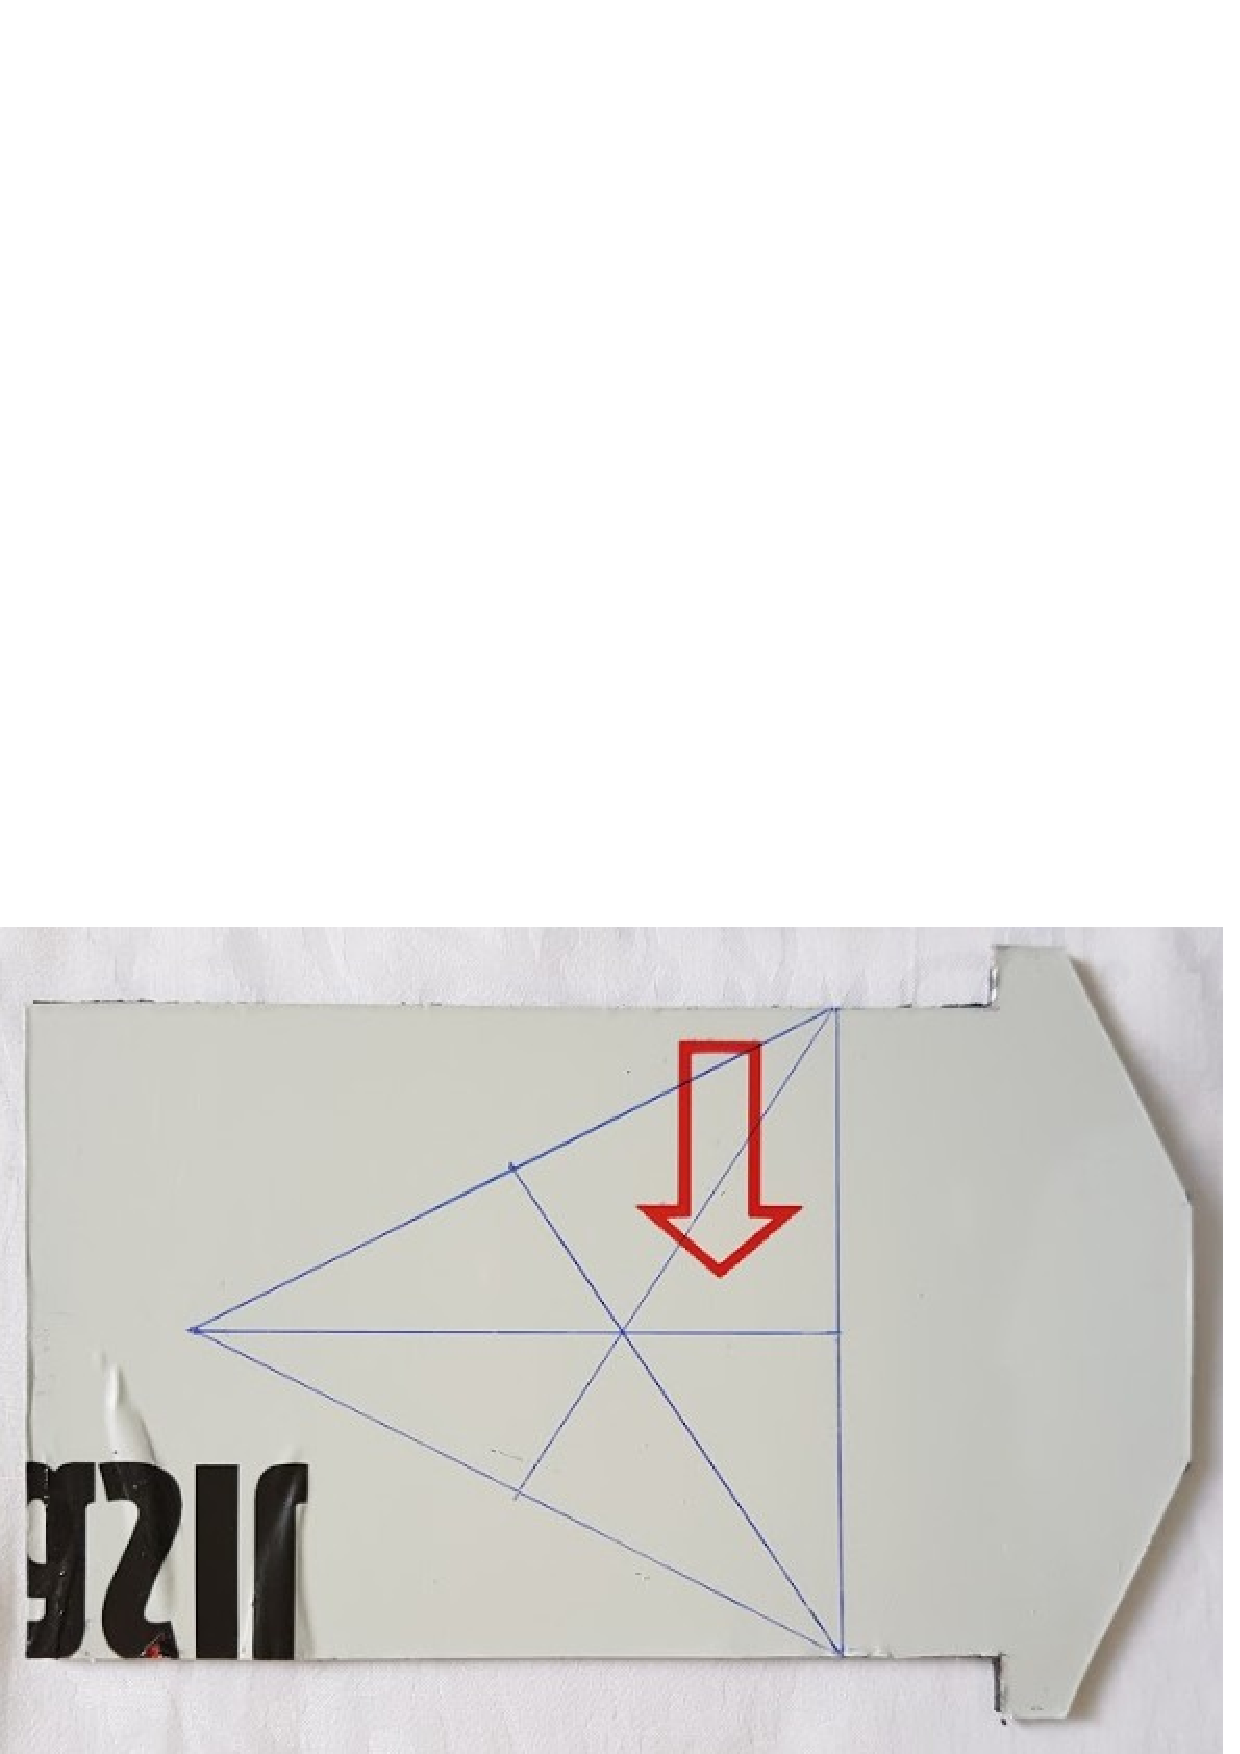
\includegraphics[width=\textwidth]{figure-02.png}
  \caption{Cantidad de publicaciones por año.}
  \label{fig-02}
  \source{Elaboración propia.}
  \end{minipage}
\end{figure}

\begin{enumerate}[label=\textbf{PI\arabic*}]
\setcounter{enumi}{1}
\item
  \textbf{Características de las publicaciones de organismos
  internacionales acerca de la transformación digital en el ámbito de la
  educación superior}
\end{enumerate}

En cuanto a los países de adscripción de los autores y sedes de los OI,
se distinguió que la distribución de la producción de literatura
proviene esencialmente de siete países (Argentina, Chile, EE. UU.,
Federación de Rusia, Francia, Panamá y Senegal), siendo Francia el de
mayor producción; la totalidad de la literatura hallada de la CEPAL
procede de Chile y una de ellas está en coautoría con las Naciones
Unidas y la Unesco. Asimismo, se identificó que este último OI cuenta
con presencia en diversos países. Además, en cinco documentos de la BID
y uno de la OEI no se declara el país de publicación (\Cref{tab-08}).

\begin{table}[htpb]
\centering
\begin{threeparttable}
\caption{distribución de la bibliografía, según el país de publicación.}
\label{tab-08}
\begin{tabular}{*{8}{l}}
\toprule
  País de la publicación & \multicolumn{6}{c}{Organismos internacionales} & Total \\
\midrule
  No especifica & 5 & & & 1 & & & 6 \\
  Chile & & 6 & & & & & 6 \\
  Francia & & 1 & 4 & & & 3 & 8 \\
  Argentina & & & & 1 & & & 1 \\
  Panamá & & 1 & & & & & 1 \\
  EE. UU. & & & & & 1 & & 1 \\
  Senegal & & & & & & 1 & 1 \\
  Federación de Rusia & & & & & & 1 & 1 \\
  Total & 5 & 8 & 4 & 2 & 1 & 5 & 25 \\
 \bottomrule
\end{tabular}
\source{Elaboración propia.}
\begin{tablenotes}
\small {
	\item{Nota: la CEPAL tiene una publicación con tres países de publicación (Chile, Francia y Panamá).} 
    }
\end{tablenotes}
\end{threeparttable}
\end{table}

Referente al idioma, el inglés es el principal lenguaje de producción
con 44\% de los documentos seleccionados como relevantes, seguido de
inglés y español (30\%), y en menor porcentaje, en español (26\%).
Específicamente, la Unesco se caracterizó por publicar fundamentalmente
en el idioma inglés y la OEI, solo en español (\Cref{tab-09}).


\begin{table}[htpb]
  \centering
  \caption{Idiomas de las publicaciones.}
  \label{tab-09}
  \begin{tabular}{llllllll}
  \toprule
  Idioma & \multicolumn{7}{c}{Organismos internacionales} \\
    & BID & CEPAL & OCDE & OEI & ONU & Unesco & Total \\
  \midrule
  Inglés & 0 & 2 & 3 & 0 & 1 & 4 & 10 \\
  Español & 2 & 2 & 0 & 2 & 0 & 0 & 6 \\
  Inglés y español & 3 & 2 & 1 & 0 & 0 & 1 & 7 \\
  Total & 5 & 6 & 4 & 2 & 1 & 5 & 23 \\
  \bottomrule
  \end{tabular}
  \source{Elaboración propia.}  
\end{table}

En cuanto a tipo de recurso o material de las publicaciones, destacaron
los libros con 48\%, seguido de documentos de programa o de reunión
(13\%) y capítulos de libro (13\%) y en menor cantidad, informes (9\%),
revistas, diarios y boletines informativos (9\%), así como notas
técnicas (8\%). Particularmente, el BID produjo más de estos últimos
tres tipos; la CEPAL se enfocó a recursos de tipo libro y la OCDE a
capítulos de libro. Estos enfoques reflejan una audiencia que abarca
desde académicos e investigadores hasta líderes de políticas y
ejecutivos en el ámbito educativo.

\begin{enumerate}[label=\textbf{PI\arabic*}]
\setcounter{enumi}{2}
\item
  \textbf{Contextos de estudio sobre la transformación digital en la
  educación superior en los que se han enfocado los organismos
  internacionales}
\end{enumerate}

Con respecto a la tercera pregunta, los estudios de los OI se
contextualizaron en América Latina y el Caribe, Asia, Oriente Medio,
África Oriental y algunos países de Europa. En específico, la Unesco
abordó el tema de la transformación digital en la educación terciaria en
la mayoría de las zonas geográficas mencionadas, a excepción de Europa,
en el cual se estudiaron los escenarios de transformación en Hungría,
Italia y Letonia por la OCDE. Asimismo, se destaca que la mayoría de los
OI se enfocaron en los contextos geográficos de América Latina y el
Caribe, y la ONU se centró en entornos a nivel global. En la \Cref{fig-03} se
muestra lo descrito y entre paréntesis la cantidad de publicaciones por
OI.

\begin{figure}[htpb]
  \centering
  \begin{minipage}{.8\textwidth}
  
\includegraphics[width=\textwidth]{figure-03.png}
  \caption{Contextos geográficos de estudio.}
  \label{fig-03}
  \source{Elaboración propia.}
  \end{minipage}
\end{figure}

En América Latina, se mencionan un total de 13 países en diferentes
combinaciones. Los más recurrentes son Argentina, Brasil, Chile,
Colombia y México. Otros países incluidos son Perú, Uruguay, Bolivia,
Ecuador, El Salvador, Honduras, Panamá y Costa Rica. En el Caribe, se
mencionan 12 países o zonas, entre ellos Aruba, Barbados, Belice, Islas
Vírgenes Británicas, Granada, Guyana, Jamaica, Santa Lucía, San Vicente
y las Granadinas, Trinidad y Tobago, Antigua y Barbuda, y Santa Lucía.
En total, la región de América Latina y el Caribe fue la más estudiada
(16 publicaciones de 23) y por la mayoría de los OI.

Con respecto al continente africano, en un estudio de la Unesco (03U) lo
refirieron de manera general y en otro documento del mismo organismo
(04U), se enfocaron en países como Chad, Madagascar, Nigeria, Ruanda y
Tunisia. La ONU y la Unesco describen un conjunto diverso de países a
nivel global que incluyen naciones de Europa, Asia y Medio Oriente.
Entre los mencionados están Albania, Bulgaria, Grecia, Polonia,
Portugal, Reino Unido y República Checa en Europa; Arabia Saudita,
Azerbaiyán, Bahrein, Emiratos Árabes Unidos, Omán y Qatar en Medio
Oriente; y Bangladesh, China, Kazajstán, Kirguistán y Malasia en Asia.
También incluye a Finlandia y Ucrania, lo cual refleja una cobertura
geográfica amplia que resalta la diversidad de contextos culturales y
económicos en los cuales la ONU y la UNESCO promueven iniciativas
globales.

\begin{enumerate}[label=\textbf{PI\arabic*}]
\setcounter{enumi}{3}
\item
  \textbf{Líneas temáticas de la transformación digital en la educación
  superior en las que se han enfocado los organismos internacionales}
\end{enumerate}

Con respecto a la última pregunta, se hizo una clasificación de las
palabras clave, las cuales resultaron en seis categorías de análisis: 1)
aspectos tecnológicos, 2) aspectos educativos, 3) aspectos
organizacionales, 4) aspectos sociales, 5) de contexto, 6) de
habilidades y competencias. Es relevante aclarar que, únicamente el BID
y la Unesco incluyeron palabras clave en sus publicaciones, lo que
representó el 30\% del corpus bibliográfico (\Cref{tab-10}).


\begin{table}[htbp]
    \centering
    \small
    \caption{Perspectivas de análisis de la transformación digital por OI, según palabras clave.}  
    \label{tab-10}
    \begin{tabular}{
    >{\raggedright\arraybackslash}p{0.17\textwidth}
    ll
    >{\raggedright\arraybackslash}p{0.38\textwidth}
    l}
    \toprule
    Perspectivas de análisis & OI & ID & Palabras clave & Frecuencia\\
    \midrule
  \multirow{5}{=}{Aspecto tecnológico} & \multirow{2}{*}{BID} &
      04BID & Transformación digital & 1 \\
      & & 01BID & Digitalización & 1 \\
      & \multirow{3}{*}{Unesco} & 03U, 04U & Tecnología de la información &
      2 \\
      & & 03U, 04U & Iniciación a la informática & 2 \\
      & & 03U & Inteligencia artificial & 1 \\
      \multirow{10}{=}{Aspecto educativo} & \multirow{4}{*}{BID} &
      01BID & Educación & 1 \\
      & & 02BID & Educación 4.0 & 1 \\
      & & 04BID & Educación híbrida & 1 \\
      & & 04BID & Innovación educativa & 1 \\
      & \multirow{6}{*}{Unesco} & 02U & Innovación educacional & 1 \\
      & & 01U, 04U, 05U & Enseñanza técnica y profesional & 3 \\
      & & 05U & Enseñanza superior & 1 \\
      & & 02U & Cooperación educacional & 1 \\
      & & 01U, 04U, 05U & Tecnología educacional & 3 \\
      & & 02U & Aprendizaje en línea & 1 \\
      \multirow{3}{=}{Habilidades y competencias} & BID & 04BID &
      Habilidades S21 & 1 \\
      & \multirow{2}{*}{Unesco} & 04U & Desarrollo de las habilidades & 1 \\
      & & 03U & Competencia profesional & 1 \\
      \multirow{4}{=}{Aspecto organizacional} & BID & 01BID &
      Instituciones educativas & 1 \\
      & \multirow{3}{*}{Unesco} & 02U & Proyecto de educación & 1 \\
      & & 02U & Alianza público-privada & 1 \\
      & & 02U & Financiación de la educación & 1 \\
      \multirow{4}{=}{Aspecto social} & BID & 01BID & Políticas
      públicas & 1 \\
      & \multirow{3}{*}{Unesco} & 03U & Funcionario público & 1 \\
      & & 01U, 05U & Estudio de caso & 2 \\
      & & 03U & Gobierno & 1 \\
      \multirow{4}{=}{Contexto} & \multirow{2}{*}{BID} & 04BID &
      América Latina y el Caribe & 1 \\
      & & 01BID & Crisis económicas & 1 \\
      & \multirow{2}{*}{Unesco} & 01BID & COVID-19 & 1 \\
      & & 01U & País en desarrollo & 1 \\
      \bottomrule
      \source{elaboración propia}
    \end{tabular}
\end{table}

Debido a que fueron escasas las publicaciones (siete de 23) que
contenían palabras clave para identificar los aspectos o perspectivas de
análisis de la transformación digital estudiados por los OI, se
revisaron los resúmenes, los objetivos, los índices y las conclusiones
de los demás documentos seleccionados. Como resultado, se realizó una
clasificación de los temas en siete categorías: 1) aspectos
tecnológicos, 2) aspectos educativos, 3) aspectos organizacionales, 4)
aspectos sociales, 5) de contexto, 6) de habilidades y competencias, y
7) la visión que se tiene sobre la transformación digital (\Cref{tab-11}).


\newpage
\begin{longtable}{
>{\raggedright\arraybackslash}p{0.2\textwidth} l >{\raggedright\arraybackslash}p{0.65\textwidth}}
\caption{Perspectivas de análisis de la transformación digital por OI, según aspectos temáticos.}
\label{tab-11}\\
\toprule
Perspectivas de análisis & OI & Aspectos temáticos en resúmenes, objetivos, índices y conclusiones.\\
\midrule
    \multirow{22}{=}{Aspecto tecnológico} & BID & Transformación
    tecnológica \\
    & \multirow{7}{*}{CEPAL} & Uso de medios digitales \\
    & & Adopción de nuevas tecnologías \\
    & & Tecnologías de la cuarta revolución industrial \\
    & & Tecnologías digitales maduras y de avanzada \\
    & & TIC \\
    & & Inversión en acceso a computadoras, Internet de banda ancha y al
    IoT \\
    & & Acceso a Internet y dispositivos habilitados para Internet \\
    & \multirow{2}{*}{OCDE} & Infraestructura digital y sistemas de datos \\
    & & Acceso y equidad en uso tecnológico \\
    & \multirow{5}{*}{OEI} & Tecnologías en la transformación digital \\
    & & Tecnologías emergentes para las Administraciones Públicas Educativas
    (APE) \\
    & & Digitalización \\
    & & Uso de las TIC \\
    & & Innovación \\
    & ONU & Estructura TIC y acceso a la tecnología \\
    & \multirow{6}{*}{Unesco} & Desarrollo técnico y tecnológico \\
    & & Conectividad e infraestructura \\
    & & Adopción de la IA \\
    & & Tecnología de la información \\
    & & Barreras estructurales: infraestructura de la Tecnología de la
    Información (TI) y de acceso a los datos \\
    & & Equipamiento renovado de herramientas tecnológicas \\
\midrule
    \multirow{18}{=}{Aspecto educativo} & \multirow{6}{*}{BID} &
    Tendencias digitales en educación \\
    & & Nuevas prácticas pedagógicas \\
    & & Virtualización de los procesos de enseñanza y aprendizaje \\
    & & Desarrollo de aprendizaje por proyecto o aula invertida \\
    & & Inclusión planificada de tecnologías en la educación \\
    & & Brechas pedagógicas \\
    & \multirow{6}{*}{CEPAL} & Fortalecimiento de la educación digital \\
    & & Medidas encaminadas a la transformación educativa \\
    & & Transformación digital de aprendizajes \\
    & & Estrategia para una educación con medios digitales \\
    & & Educación inclusiva y de calidad \\
    & & Combinación de modos de aprendizaje digital y presencial \\
    & \multirow{3}{*}{OCDE} & Uso de herramientas digitales por docentes y
    estudiantes \\
    & & Preparación, prácticas y desempeño digital \\
    & & Aprendizaje digital para todos \\
    & ONU & Desarrollo de capacidades digitales \\
    & \multirow{2}{*}{Unesco} & Enseñanza y aprendizaje utilizando
    tecnología \\
    & & Tecnología educacional \\
\midrule
    \multirow{13}{=}{Habilidades y competencias} &
    \multirow{3}{*}{BID} & Reforzamiento de competencias digitales y
    desarrollo de habilidades digitales \\
    & & Impulso hacia desarrollo de habilidades y aptitudes del siglo XXI \\
    & & Formación digital, pedagógica y de habilidades blandas \\
    & \multirow{2}{*}{CEPAL} & Desarrollo de habilidades y competencias
    digitales para el siglo XXI \\
    & & Desarrollo de habilidades digitales para el uso de las TIC \\
    & \multirow{2}{*}{OCDE} & Habilidades digitales \\
    & & Habilidades en manejo de TIC \\
    & ONU & Habilidades y competencias digitales del siglo XXI \\
    & \multirow{5}{*}{Unesco} & Marcos integrales de competencias
    digitales \\
    & & Competencia profesional \\
    & & Competencias en IA y transformación digital \\
    & & Habilidades y capacidades digitales \\
    & & Actitudes complementarias para lograr la transformación digital de
    manera eficaz \\
\midrule
    \multirow{39}{=}{Aspecto organizacional} &
    \multirow{12}{*}{BID} & Flexibilización y agilización de los sistemas de
    formación \\
    & & Modalidades de enseñanza en remoto o híbridas \\
    & & Enfoque multifuncional de toda la institución, apoyado por una
    gestión del cambio, consultas y un liderazgo sólido \\
    & & Desarrollo de madurez digital en actitudes, capacidades, sistemas y
    procesos \\
    & & Digitalización de los sistemas educativos y oferta académica \\
    & & Ampliación de modelos de aprendizaje \\
    & & Reforzamiento de equipamiento, conectividad, plataformas y
    contenidos curriculares \\
    & & Modelo de negocio ``business to university'' \\
    & & Diseño de nuevas metodologías educativas \\
    & & Global Alumni: Modelo formativo en innovación y tecnología \\
    & & Educación basada en el \emph{e-learning} y \emph{b-learning} \\
    & & Brecha de capacidad digital en las universidades \\
    & \multirow{10}{*}{CEPAL} & Gestión de la educación \\
    & & Reestructuración de los sistemas educativos \\
    & & Financiamiento de la transformación digital en la educación \\
    & & Áreas necesarias de inversión: infraestructura física, recursos o
    materiales educativos y habilidades digitales \\
    & & Procesos de innovación \\
    & & Procesos de transformación digital en educación superior \\
    & & Oferta de programas educativos enfocados en áreas relacionadas con
    la digitalización \\
    & & Oferta de cursos relacionadas con tecnología avanzada \\
    & & Capacitación docente para optimizar el uso de las tecnologías \\
    & & Transformación de los programas educativos para la sostenibilidad
    del cambio \\
    & \multirow{8}{*}{OCDE} & Evaluación de la digitalización en la
    educación superior \\
    & & Entorno y cultura digital institucional \\
    & & Recursos financieros y humanos dedicados a infraestructura y
    sistemas digitales \\
    & & Prospectiva estratégica hacia un futuro digital \\
    & & Desarrollo (y redesarrollo) de estrategias resilientes, adaptables y
    exitosas. \\
    & & Innovación en las IES \\
    & & Emprendimiento en las IES \\
    & & Desarrollo de los procesos en docencia, investigación y
    compromiso \\
    & \multirow{2}{*}{OEI} & Ecosistemas \emph{fintech} (finanza y
    tecnología) \\
    & & Análisis de la transformación digital en la gestión educativa \\
    & \multirow{2}{*}{ONU} & Sistemas educativos dinámicos \\
    & & Financiación de tecnología para el desarrollo sostenible \\
    & \multirow{5}{*}{Unesco} & Recomendaciones para impulsar la
    transformación digital \\
    & & Barreras culturales: cultura y liderazgo de innovación \\
    & & Barreras organizacionales: estructuras y los procesos jerárquicos
    rígidos en la innovación \\
    & & Formación digital para docentes, instructores, ejecutivos y
    directivos \\
    & & Política continua y organizada sobre tecnología digital en la
    educación y formación técnica y vocacional (TVET, por sus siglas en
    inglés) \\
\midrule
    \multirow{27}{=}{Aspecto social} & \multirow{5}{*}{BID} &
    Acciones y políticas para potenciar la expansión de las nuevas
    modalidades de oferta educativa \\
    & & Brechas digitales \\
    & & Desarrollo de una ciudadanía del futuro con competencias digitales y
    habilidades interpersonales \\
    & & Desarrollo de habilidades y competencias digitales alineadas al
    mercado laboral \\
    & & Recomendaciones de políticas educativas \\
    & \multirow{9}{*}{CEPAL} & Articulación con sectores de política
    pública \\
    & & Revisión del estado de la transformación digital en el sector
    social \\
    & & Cultura de innovación \\
    & & Privacidad de datos y ciberseguridad \\
    & & Inclusión digital \\
    & & Utilización de la tecnología digital considerando su impacto
    social \\
    & & Recomendaciones para mejorar la financiación de educación de calidad
    e infraestructura resiliente \\
    & & Recomendaciones para responsables de formulación de políticas \\
    & & Medidas para una reconstrucción educativa inclusiva y
    transformadora \\
    & \multirow{6}{*}{OCDE} & Fomento de la inclusión y sustentabilidad \\
    & & Adopción de nuevas tecnologías en las empresas \\
    & & Recomendaciones de políticas públicas y educativas para fortalecer
    el marco de digitalización en la educación superior \\
    & & Recomendaciones a responsables de políticas y los líderes de las
    IES \\
    & & Acciones en general para la transformación digital \\
    & & Usuarios beneficiados: estudiantes, graduados y empleadores \\
    & \multirow{2}{*}{OEI} & Organizaciones públicas \\
    & & Economía del conocimiento \\
    & \multirow{2}{*}{ONU} & Adquisición de nuevas tecnologías innovadoras
    para generar capital humano competitivo \\
    & & Desarrollo de habilidades y posibilidades laborales adecuadas en el
    siglo XXI \\
    & \multirow{3}{*}{Unesco} & La transformación digital en la TVET como
    apoyo a la sostenibilidad y la resiliencia de las sociedades \\
    & & Capacidad y cultura, costo y sustentabilidad, contenido y currículo
    o planes de estudio, coordinación y liderazgo \\
    & & Fortalecimiento de las habilidades digitales para mejorar la
    empleabilidad \\
\midrule
    \multirow{10}{=}{Contexto} & \multirow{3}{*}{BID} &
    Globalización \\
    & & Cuarta revolución industrial \\
    & & Tendencias en el mercado laboral \\
    & \multirow{3}{*}{CEPAL} & Efectos de la transformación digital \\
    & & La educación en la región, previo y durante la crisis sanitaria
    ocasionada por la COVID-19 \\
    & & Cuarta revolución industrial \\
    & OEI & Tendencias en el mercado laboral \\
    & ONU & Respuesta al Covid-19 \\
    & \multirow{2}{*}{Unesco} & Sistemas educativos afectados e impactados
    por la pandemia de COVID-19 \\
    & & Prácticas y tendencias en transformación digital en la TVET en
    países en desarrollo \\
\midrule
    \multirow{9}{=}{Visión de la TD} & BID & Planteamiento de
    transformaciones holísticas en la oferta educativa en las instituciones
    de educación postsecundaria \\
    & \multirow{2}{*}{CEPAL} & Visión holística y transformadora de los
    desafíos educativos \\
    & & Desarrollo del ecosistema digital en la educación superior o
    terciaria en tecnologías digitales desde la visión organizativa,
    pedagógico y de innovación \\
    & \multirow{2}{*}{OCDE} & Desarrollar una estrategia coordinada que
    tenga en cuenta todos los aspectos de la digitalización y proporcionar y
    promover una visión integral \\
    & & Visión estratégica de la transformación digital de manera holística
    y coherente \\
    & OEI & Dimensiones prioritarias para la transformación digital en las
    Administraciones Públicas Educativas \\
    & ONU & Enfoque holístico para la transformación del gobierno digital \\
    & \multirow{2}{*}{Unesco} & Factores habilitantes para la transformación
    digital en TVET \\
    & & Niveles del marco conceptual de transformación digital en TVET \\
    \bottomrule
    \source{elaboración propia}
\end{longtable}



En conjunto, la visión que se tiene sobre la transformación es promover
cambios de manera integral o bajo un enfoque holístico y coherente en
las instituciones de formación universitaria, así como en las de
formación técnica y vocacional, en donde se plateen estrategias
coordinadas que abarquen las dimensiones de lo organizativo, pedagógico
y de innovación en el ecosistema digital.

En la implementación de soluciones tecnológicas en las instituciones
educativas, se destacan la modernización de infraestructuras digitales y
sistemas de datos, la adopción y uso equitativo de tecnologías avanzadas
como la inteligencia artificial y tecnologías de la cuarta revolución
industrial, así como el desarrollo de conectividad robusta, y la
superación de barreras de infraestructura y el acceso a dispositivos e
internet de banda ancha.

En lo educativo, incluyen la virtualización de procesos de enseñanza y
aprendizaje, el desarrollo de nuevas prácticas pedagógicas como el aula
invertida, y la inclusión estratégica de tecnologías para cerrar brechas
pedagógicas. También, la capacitación docente para el uso óptimo de
herramientas digitales y la combinación de modalidades de aprendizaje
presencial y digital, con el fin de lograr una educación inclusiva,
accesible y de calidad.

Se destaca el reforzamiento y desarrollo de habilidades y competencias
digitales clave, tales como destrezas en el manejo de TIC y en
inteligencia artificial, junto con marcos integrales que aborden
habilidades del siglo XXI, como la adaptación tecnológica y el
pensamiento crítico. Además, se priorizan actitudes proactivas y
competencias profesionales que integren formación digital, pedagógica y
habilidades blandas, esenciales para una implementación efectiva de la
transformación digital.

Organizacionalmente, la transformación busca crear entornos digitales,
superar brechas de capacidad digital y fomentar una cultura de
innovación adaptativa. Se enfatiza la inversión en infraestructura,
programas en tecnología avanzada y políticas de digitalización
sostenibles para superar barreras organizacionales y culturales.

Desde lo social, se prioriza la reducción de brechas digitales, la
inclusión y la preparación para la economía del conocimiento, mediante
la promoción de habilidades alineadas al mercado laboral, la
ciberseguridad, y la colaboración en políticas públicas para una
innovación inclusiva y sostenible.

% !TeX root = main.tex
\section{Reflexiones finales y conclusiones}\label{sec-reflexiones-finales-y-conclusiones}

En el marco de los resultados presentados, se destaca que abordar la
transformación digital conlleva a comprenderla como un proceso de
integración tecnológica digital en varias áreas de una organización,
tanto internas como externas, y se compone de un marco complejo de
cambios que involucra tecnologías digitales y emergentes,
infraestructura, modelos educativos, gestión educativa, desarrollo de
competencias digitales y política pública, y que converge en cuatro
dimensiones clave: tecnológica, organizacional, educacional y social.
Este enfoque sugiere que las instituciones educativas requieren un
análisis holístico y los hallazgos coinciden con lo señalado por \textcite{aditya2021,bikse2021} y \textcite{benavides2020-castro} para garantizar la transformación digital en las
IES.

Si bien, los OI presentan publicaciones desde todas las perspectivas
mencionadas ---excepto la OEI que solo se enfocó en lo tecnológico,
organizacional y social---, y el BID, la CEPAL, la OCDE y la ONU
presentan la transformación como una visión holística, el tema en la
educación superior ha sido estudiada e implementada de manera segmentada
y con un abordaje desde lo empresarial y comercial. Por ejemplo, la
promoción del modelo ``business to university'', los ecosistemas
\emph{Fintech} (finanza y tecnología) y el financiamiento para el
emprendimiento, así como la generación de capital humano competitivo en
aras de mejorar la empleabilidad y asegurar que los principales
beneficiarios de estos esfuerzos sean los estudiantes, graduados y
empleadores.

No obstante, los abordajes novedosos en los que se trata el tema y
pueden guiar futuras líneas de estudio están relacionadas con el
desarrollo de estrategias resilientes y programas educativos sostenibles
para un futuro digital, así como la promoción de prácticas pedagógicas
centradas en la inclusión de tecnologías para la reducción de brechas
pedagógicas y digitales mediante la transformación digital. Además, se
reconoció que tres cuartas partes de los enfoques identificados en los
OI revisados, están concentrados en procesos de evaluación, y que menos
de la mitad plantean propuestas de solución, iniciativas o proyectos.
Esto conlleva también a pensar en otras líneas de investigación
relacionadas con el desarrollo de programas y estrategias integrales de
la transformación digital en las IES, donde se consideren todas las
áreas y actores clave para su implementación en las universidades.

En suma, esto concuerda con lo puntualizado por \textcite{cerdá-suárez2021}, al señalar que estudiar este fenómeno complejo y
de interés actual para las universidades, tanto en países más avanzados
como en vías de desarrollo y particularmente en la región de América
Latina y el Caribe, es necesario tomar en cuenta una serie de elementos
para su implementación. Estos van desde la formulación de políticas y
agendas nacionales que respalden la transformación en el país hasta el
fomento de habilidades digitales, tanto en profesores como en
estudiantes y atender cuestiones de accesibilidad y equidad.

En conclusión, no se puede desestimar que el tema de la transformación
digital en el ámbito educativo, ha sido significativamente acelerado por
la pandemia de COVID-19 y que ha propiciado la necesidad global por
implementarlo en las instituciones educativas, así como el interés de
diversos OI por analizarlo desde múltiples perspectivas, enfoques y
contextos geográficos en el mundo, con el fin de impulsarla y ofrecer
una caracterización amplia del tema para una mayor comprensión de la
misma en la educación.

Si bien el MSL posibilita la exploración de publicaciones sobre un tema
de interés, sus limitaciones en este estudio están relacionadas con el
nivel general de análisis, por lo que no se ahondó en los marcos
conceptuales. Sin embargo, este enfoque resulta útil para seleccionar
documentos que permitan un análisis más profundo en una siguiente fase,
como se recomienda en la revisión sistemática de la literatura.
Asimismo, debido a que escasas publicaciones contenían palabras clave (7
de 23), fue necesario revisar información adicional en la sección de
resumen, objetivos, índices y conclusiones, por lo que, requirió de más
tiempo en la revisión de cada documento para determinar su potencial
relevancia.

No obstante, se reconoce que el MSL es una herramienta valiosa para
comprender el panorama actual del conocimiento, identificar áreas de
investigación prioritarias y respaldar la toma de decisiones
fundamentadas en el ámbito de la educación digital. El análisis de 23
documentos, posibilitó la clasificación de perspectivas temáticas, tipos
de aportes y enfoques de investigación, así como ubicar los contextos
geográficos analizados y vislumbrar futuras líneas de indagación. Por
consiguiente, este artículo proporciona el procedimiento metodológico
particular para publicaciones no catalogadas como científicas pero que
aportan al campo de conocimiento, y un marco referencial de cómo ha sido
la producción documental a nivel internacional en lo referente a la
transformación digital en el ámbito de la educación superior, desde la
perspectiva de seis OI.



\section{Agradecimientos}\label{sec-agradecimientos}

La investigación presentada en este documento fue financiada a través del Sistema Nacional de Posgrados (SNP) del Consejo Nacional de Humanidades, Ciencias y Tecnologías (CONAHCYT), como parte de la tesis generada en el Doctorado en Ciencias Educativas (IIDE) de la Universidad Autónoma de Baja California (UABC). 



\printbibliography\label{sec-bib}
%conceptualization,datacuration,formalanalysis,funding,investigation,methodology,projadm,resources,software,supervision,validation,visualization,writing,review
\begin{contributors}[sec-contributors]

\authorcontribution{Vannessa Lucía Sandoval-Benavides
}[conceptualization,datacuration,formalanalysis,methodology,writing,visualization]
\authorcontribution{Maricela López-Ornelas
}[conceptualization,supervision,validation,review]
\end{contributors}
\end{document}
